\graphicspath{{capitulos/Capitulo5-Resultados-experimentales/recursos/}}

\section{Resultados experimentales} \label{capitulo:5}
%En este capítulo se detallan los casos de prueba empleados para la parte de experimentación realizada para este TFM. La metaheurística de la \fasedos{} del sistema (definida en la \autoref{sec:3:metaheurística}) consta de un conjunto de parámetros, enumerados en esta sección, que afectan al rendimiento de esta. Se ha analizado para cada caso, los valores de cada parámetro que mejores resultados ofrecen.

En este capítulo se detallan los procesos realizados para la parte de experimentación realizada en este TFM. En primer lugar se definen los casos de prueba empleados, posteriormente se detalla el proceso de ajuste de los parámetros, presente en toda metaheurística y que nos permite fijar los valores del VNS empleado en la \fasedos{} del sistema (definida en la \autoref{sec:3:metaheurística}) a aquellos que ofrecen mejores resultados. Por último, se ha hecho una comparación de rendimiento de la metaheurística implementada frente a la ya mencionada metaheurística \sa{}.

Las ejecuciones presentadas a lo largo de este capítulo han sido realizadas en un ordenador con las características recopiladas en la \autoref{table:5:caracteristicas-pc}.

\begin{table}[h]
	\centering
	\caption{Características del ordenador empleado para la experimentación}
	\begin{tabular}{lcc}
		\hline
		Procesador   & Intel Core i7 &  \\
		Memoria      &     16GB      &  \\
		Version Java &    JDK 8.1    &  \\ \hline
		             &               &
	\end{tabular}
\label{table:5:caracteristicas-pc}
\end{table}

\subsection{Definición de los casos de prueba}
\label{sec:5:def-casos}

Para este capítulo se han utilizado un conjunto de casos (instancias) de prueba reales que fueron proporcionados por CRIDA. Inicialmente CRIDA proporcionó información en los formatos de ficheros propuesto (véase \autoref{sec:4:req-io}) que fue adaptada para conformar los 8 casos de prueba distintos que se han empleado y definiremos a continuación. Una descripción de los casos de prueba se encuentra incluida en el \autoref{Anexo:tabla-casos}, junto con una tabla resumen de los casos que permite ver de forma más detallada y clara las características de cada uno de ellos.

Los casos de prueba van del 1 al 9, a excepción del caso 2, para el que \gls{CRIDA} no facilitó todos los datos y se decidió mantener el número identificativo de los demás casos por si en un futuro se completase con la información restante.

Los casos prueban el sistema empleando distintas Unidades de Control: Madrid, Barcelona y Palma de Mallorca; variando en cada uno el problema a resolver: modificación de la sectorización, baja (y alta en algún caso) de un controlador, o incluso ambos.

Los casos 4 y 7 resuelven los dos problemas a la vez: el cambio de sectorización y baja+alta de un controlador, por lo que son las instancias del problema más costosas de todas, y como veremos, son las que peores resultados alcanzan. % TODO: verificar que esto es cierto

Por otro lado, cabe destacar que los casos 5 requiere del uso de un controlador imaginario (para la inicialización realizada en la \faseuno{}), el caso 7 requiere de cuatro (3 para un nuevo sector, 1 para la baja del controlador) y el caso 8 y el 9 precisan de uno, mientras que el resto no necesitan ningún controlador imaginario para la inicialización. En los citados casos, el objetivo \ref{O1} tomará la máxima importancia hasta que alcance su valor máximo de 1, mientras que el los demás, el valor inicial de este ya es de uno, por lo que la búsqueda se dedicará exclusivamente al resto de los objetivos.


\subsection{Ajuste paramétrico}
En toda metaheurística y demás sistemas de optimización, tienen un conjunto de parámetros que pueden tomar un conjunto de posibles valores y que afectan activamente al rendimiento del sistema. Para poder fijar estos valores, se lleva a cambo un proceso denominado Ajuste Paramétrico, o \textit{Parameter Tunning}, que se puede realizar de diferentes formas.

El enfoque de inicialización \textit{off-line} consiste en fijar los valores previamente a la ejecución de la metaheurística de forma empírica para cada instancia del problema dado. Este proceso suele realizar de forma secuencial, es decir, de uno en uno. Sin embargo esta estrategia no considera las interacciones entre los parámetros y no garantiza hallar la configuración optima de los parámetros. Existen otras estrategias como \textit{Latin Hypercube}, emplear \textit{Racing Algorithms} o incluso puede ser planteado como otro problema de optimización a resolver mediante otra metaheurística.

Por otro lado se considera el enfoque de inicialización de parámetros \textit{on-line}, que permite una evolución dinámica, en tiempo de ejecución, de los valores de cada parámetro en función del rendimiento del sistema u otro criterio determinista o estocástico.

En este TFM, por ser lo más común y sencillo, se decidió emplear un enfoque \textit{off-line} de forma secuencial. Para ello, se han de ordenar los parámetros en función de su robustez, es decir, lo mucho que afecte un pequeño cambio en el parámetro al desempeño del algoritmo y, secuencialmente en ese orden, fijar el valor de todos los demás y realizar ejecuciones de la metaheurística con diferentes valores para el parámetro en cuestión para finalmente seleccionar aquel valor que mejores resultados ofrece. A continuación se repite el proceso para el siguiente parámetro, sucesivamente.
Una vez ajustados todos los parámetros, se repite el proceso desde el principio hasta que ningún parámetro cambie de valor.

Para que los datos sean más robustos y fiables, cada configuración ha sido ejecutada un total de 10 veces y se han hecho datos medios. En el \autoref{Anexo:ejemplo-ajuste-parametrico} pueden verse con detenimiento la forma de realizar el ajuste para la instancia concreta del caso 1 %TODO hacer anexo

% ALFONSO SAID:
% Empieza por aquel parámetro que creas que es menos robusto, es decir, aquel que al realizar un pequeño cambio en el parámetro pueda hacer que cambie significativamente el desempeño del algoritmo. Una vez que determines su valor más adecuado, lo fijas y analizas el segundo parámetro menos rubusto. Una vez que determines su valor más adecuado, lo fijas y analizas el tercer parámetro menos robusto. Y así sucesivamente, hasta el último y vuelves a empezar para realizar otro ciclo hasta que los parámetros no cambien o cambien muy poco. Siempre cambias un parámetro, nunca realices cambios en más de un parámetro a la vez.

\subsubsection{Parámetros del sistema} \label{sec:5:parametros-sistema}
Los parámetros del sistema, ordenados por su robustez son:
\begin{enumerate}
	\item Tipo de VNS
	\begin{enumerate}[label={},left=-1pt]
		\item Para skewed:
	\end{enumerate}
	\begin{enumerate}[label*={\arabic*}]
		\item Alpha
		\item Función de distancia 
	\end{enumerate}
	\item Estructuras de vecindad y orden
	\item Naturaleza del orden de los entornos (determinísticos o probabilísticos)
	\begin{enumerate}[label={},left=-1pt]
		\item Para Probabilístico:
	\end{enumerate}
	\begin{enumerate}[label*={\arabic*}]
		\item Probabilidad de diversificación
		\item Variación de la probabilidad de diversificación 
		\item Numero de iteraciones sin variar la probabilidad de diversificación 
	\end{enumerate}
	\item Número de iteraciones para comprobar el porcentaje de mejoría (ciclos)
	\item Porcentaje mínimo de mejoría
	\item Número máximo de iteraciones sin mejora para la búsqueda local
	\item Porcentaje mínimo de mejoría para la búsqueda local
\end{enumerate}

\subsubsection{Resultados del ajuste para cada caso}

El proceso que nos ocupa fue realizado siguiendo el procedimiento descrito anteriormente, obteniéndose los resultados que se encuentran recogidos en la \autoref{table:5:tunning-results}.

\begin{table}[h]
	\centering
	\caption{Sectorización modificada del Caso 1}
	\begin{tabular}{ccc}
		\hline
		\textbf{Núcleo}                                           & \textbf{Configuración} & \textbf{Intervalo}   \\ \hline
		\multicolumn{1}{l}{}                                      & \multicolumn{1}{l}{}   & \multicolumn{1}{l}{} \\
		\multicolumn{1}{c|}{\multirow{2}{*}{Barcelona Ruta Este}} & 3D                     & 7:30:00--15:00:00    \\
		\multicolumn{1}{c|}{}                                     & 5A                     & 7:30:00--10:30:00    \\
		\multicolumn{1}{l}{}                                      & \multicolumn{1}{l}{}   & \multicolumn{1}{l}{} \\
		Barcelona Ruta Oeste                                      & 6C                     & 10:30:00--15:00:00   \\ \hline
	\end{tabular}
	\label{table:5:tunning-results}
\end{table}

Como puede verse, por lo general la implementación de VNS que mejores resultados alcanza para la mayoría de los casos es su versión más sencilla: el \textit{VND}. No obstante, encontrarnos cuatro casos en los que la variante Basic, \textit{BVNS}, aporta resultados significativamente mejores en las soluciones que logra alcanzar el sistema. Sin embargo, tal y como muestra la \autoref{fig:caso4-tipo-orden-tiempo} las variaciones no suelen ser muy grandes entre sí, a escepción del \textit{SVNS}, que es el que peores resultados obtiene.

\begin{figure}
	\centering
	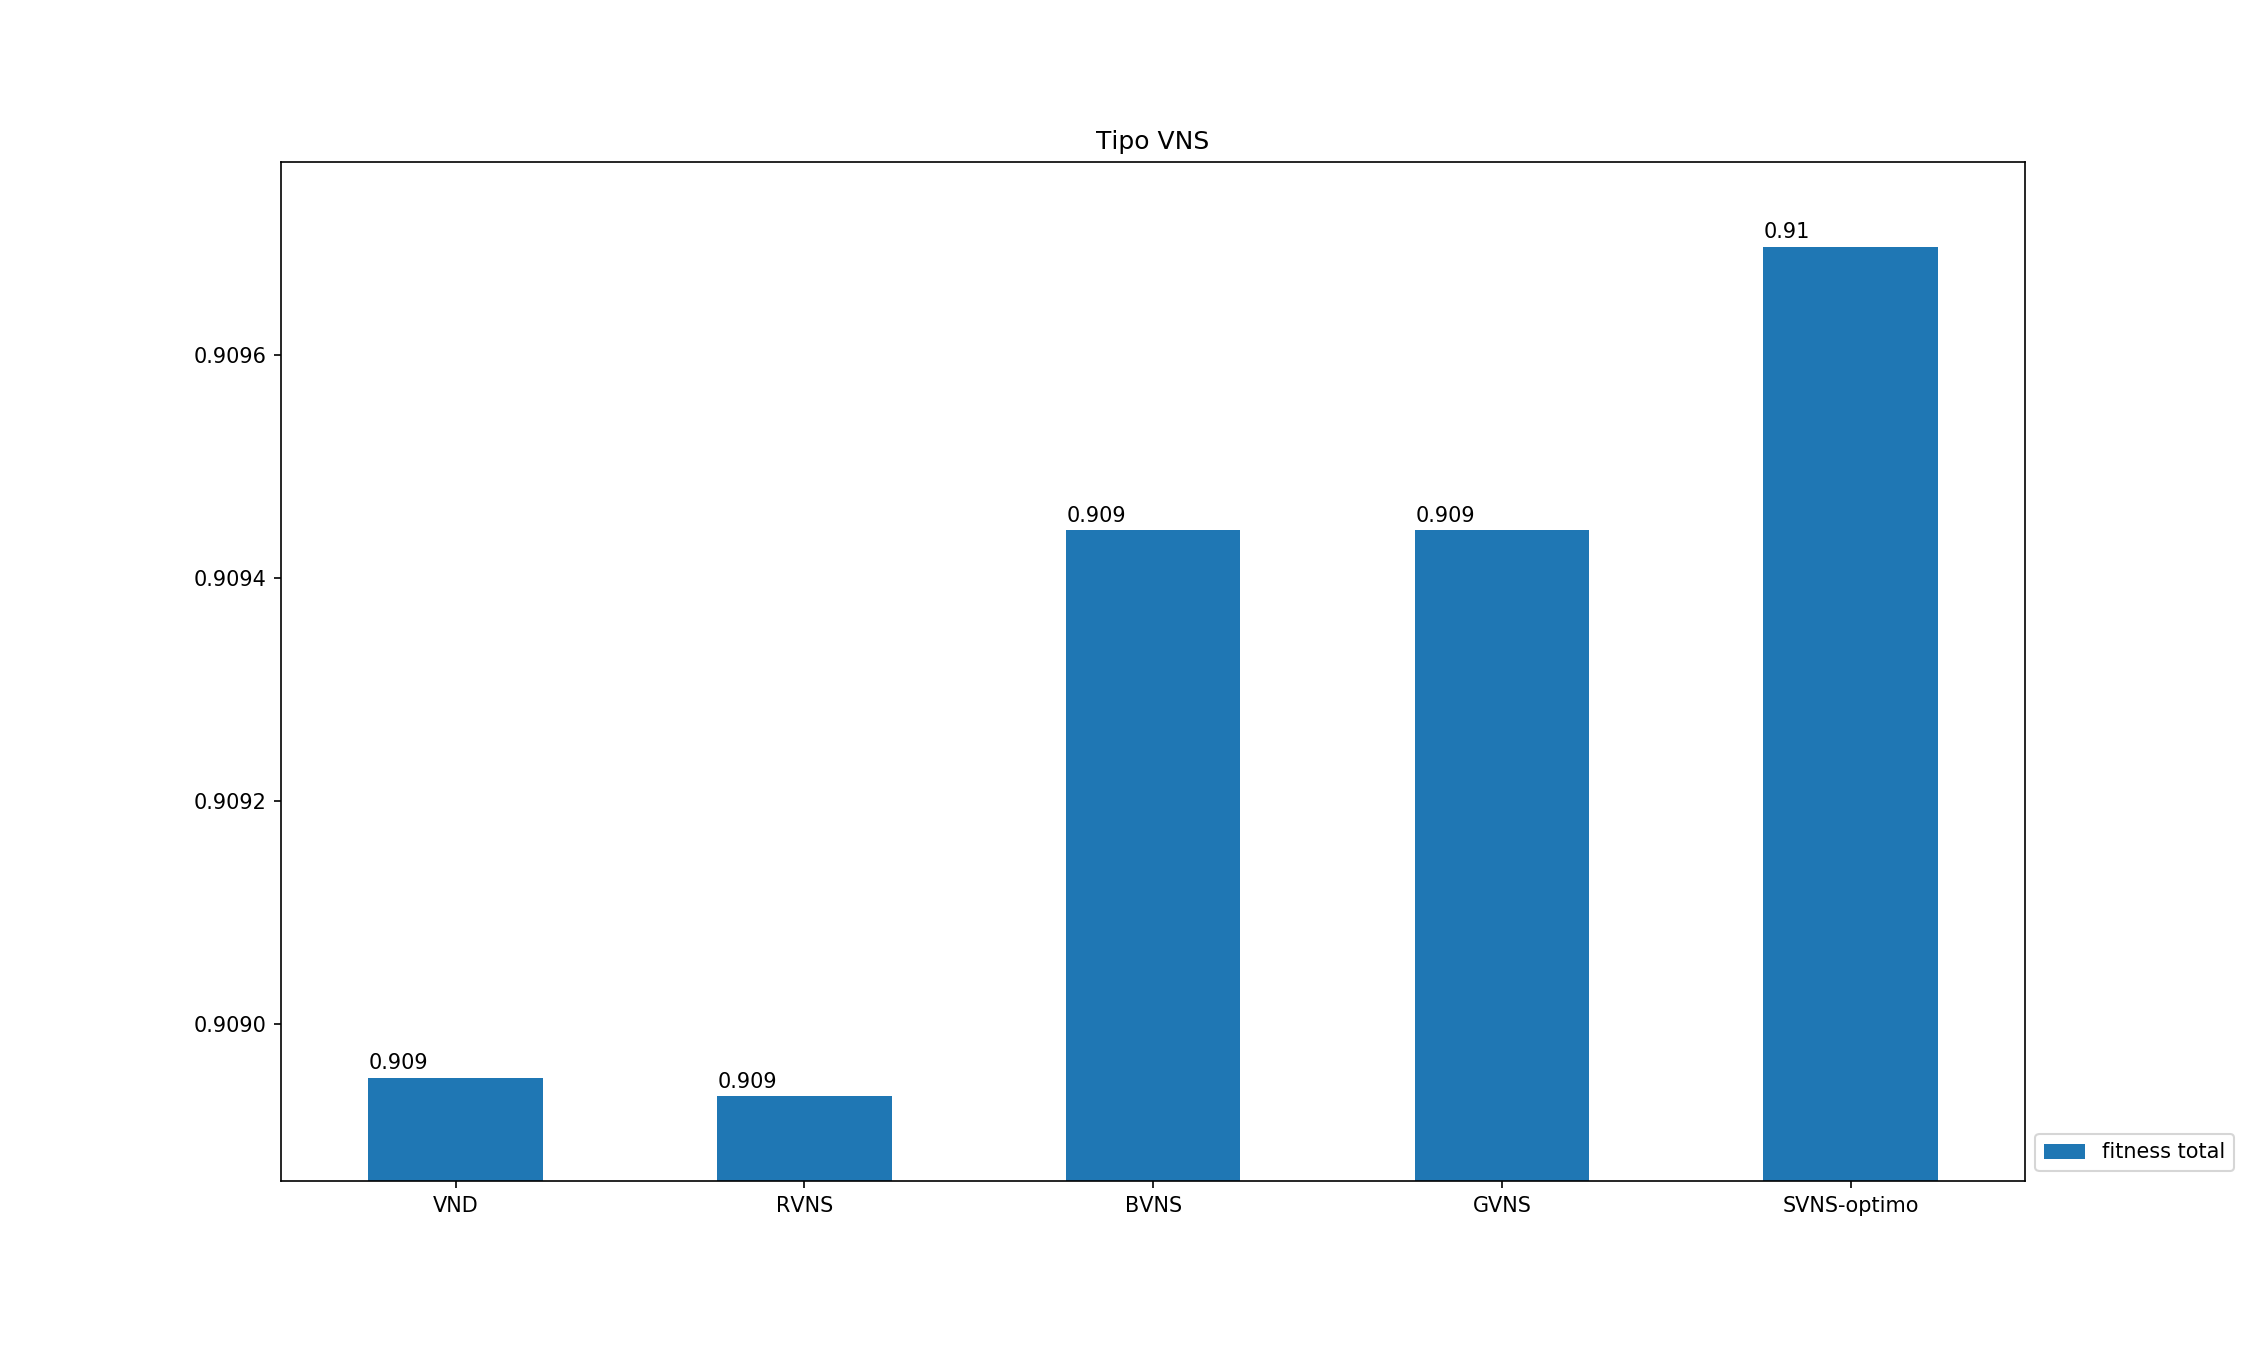
\includegraphics[width=\linewidth]{capitulos/Capitulo5-Resultados-experimentales/recursos/caso4-tipo-orden-tiempo}
	\caption{Variación del fitness según el tipo de VNS para el caso 4. Ordenado según el tiempo de ejecución de cada uno}
	\label{fig:caso4-tipo-orden-tiempo}
\end{figure}

Sin embargo, esta mejora se obtiene a costa de una mayor necesidad de tiempo de cómputo, con una diferencia de $31.2762$ segundos para el caso 4 del \textit{BVNS} frente al \textit{VND}. Sin duda hemos observado que el \textit{RVND} es el tipo de VNS que menos tiempo de cómputo requiere, pero suele ser el que peores resultados alcanza junto con el \textit{SVNS}. La \autoref{fig:caso4-tipo-orden-tiempo} ofrece adicionalmente un ranking donde nos muestra de forma ordenada los tipos de VNS que más tiempo consumen: como era de esperar, el \textit{SVNS} y el \textit{GVNS} son los más costosos, mientras que el \textit{VND} y \textit{RVNS} los que menos. Por su parte, el \textit{GVNS} y el \textit{BVNS} dan resultados que en la mayoría de los casos son muy similares entre sí, a excepción de en el caso 1 y el 3, donde los resultados son más dispares, en casos de empate, se ha optado por usar la versión menos costosa computacionalmente, que es el \textit{BVNS}.

En la \autoref{fig:caso4y9comparativa-tipos-vnsiteracion} podemos observar la evolución por iteraciones de cada VNS, donde podemos apreciar cómo, a diferencia del resto, el \textit{SVNS} no es estrictamente creciente, aceptando soluciones peores. La línea \textit{SVNS-optimo} señala la mejor solución alcanzada hasta el momento por el \textit{SVNS}, que como podemos ver, no alcanza resultados tan buenos como los del resto. Cada ejecución termina cuando se alcanza la condición de parada del porcentaje mínimo de mejora. Además, el desempeño del \textit{BVNS} y el \textit{GVNS} es el mismo en ambos casos, aunque esto no siempre sucede en todas las iteraciones ni en todos los casos.

\begin{figure}
	\begin{subfigure}{\linewidth}
		\centering
		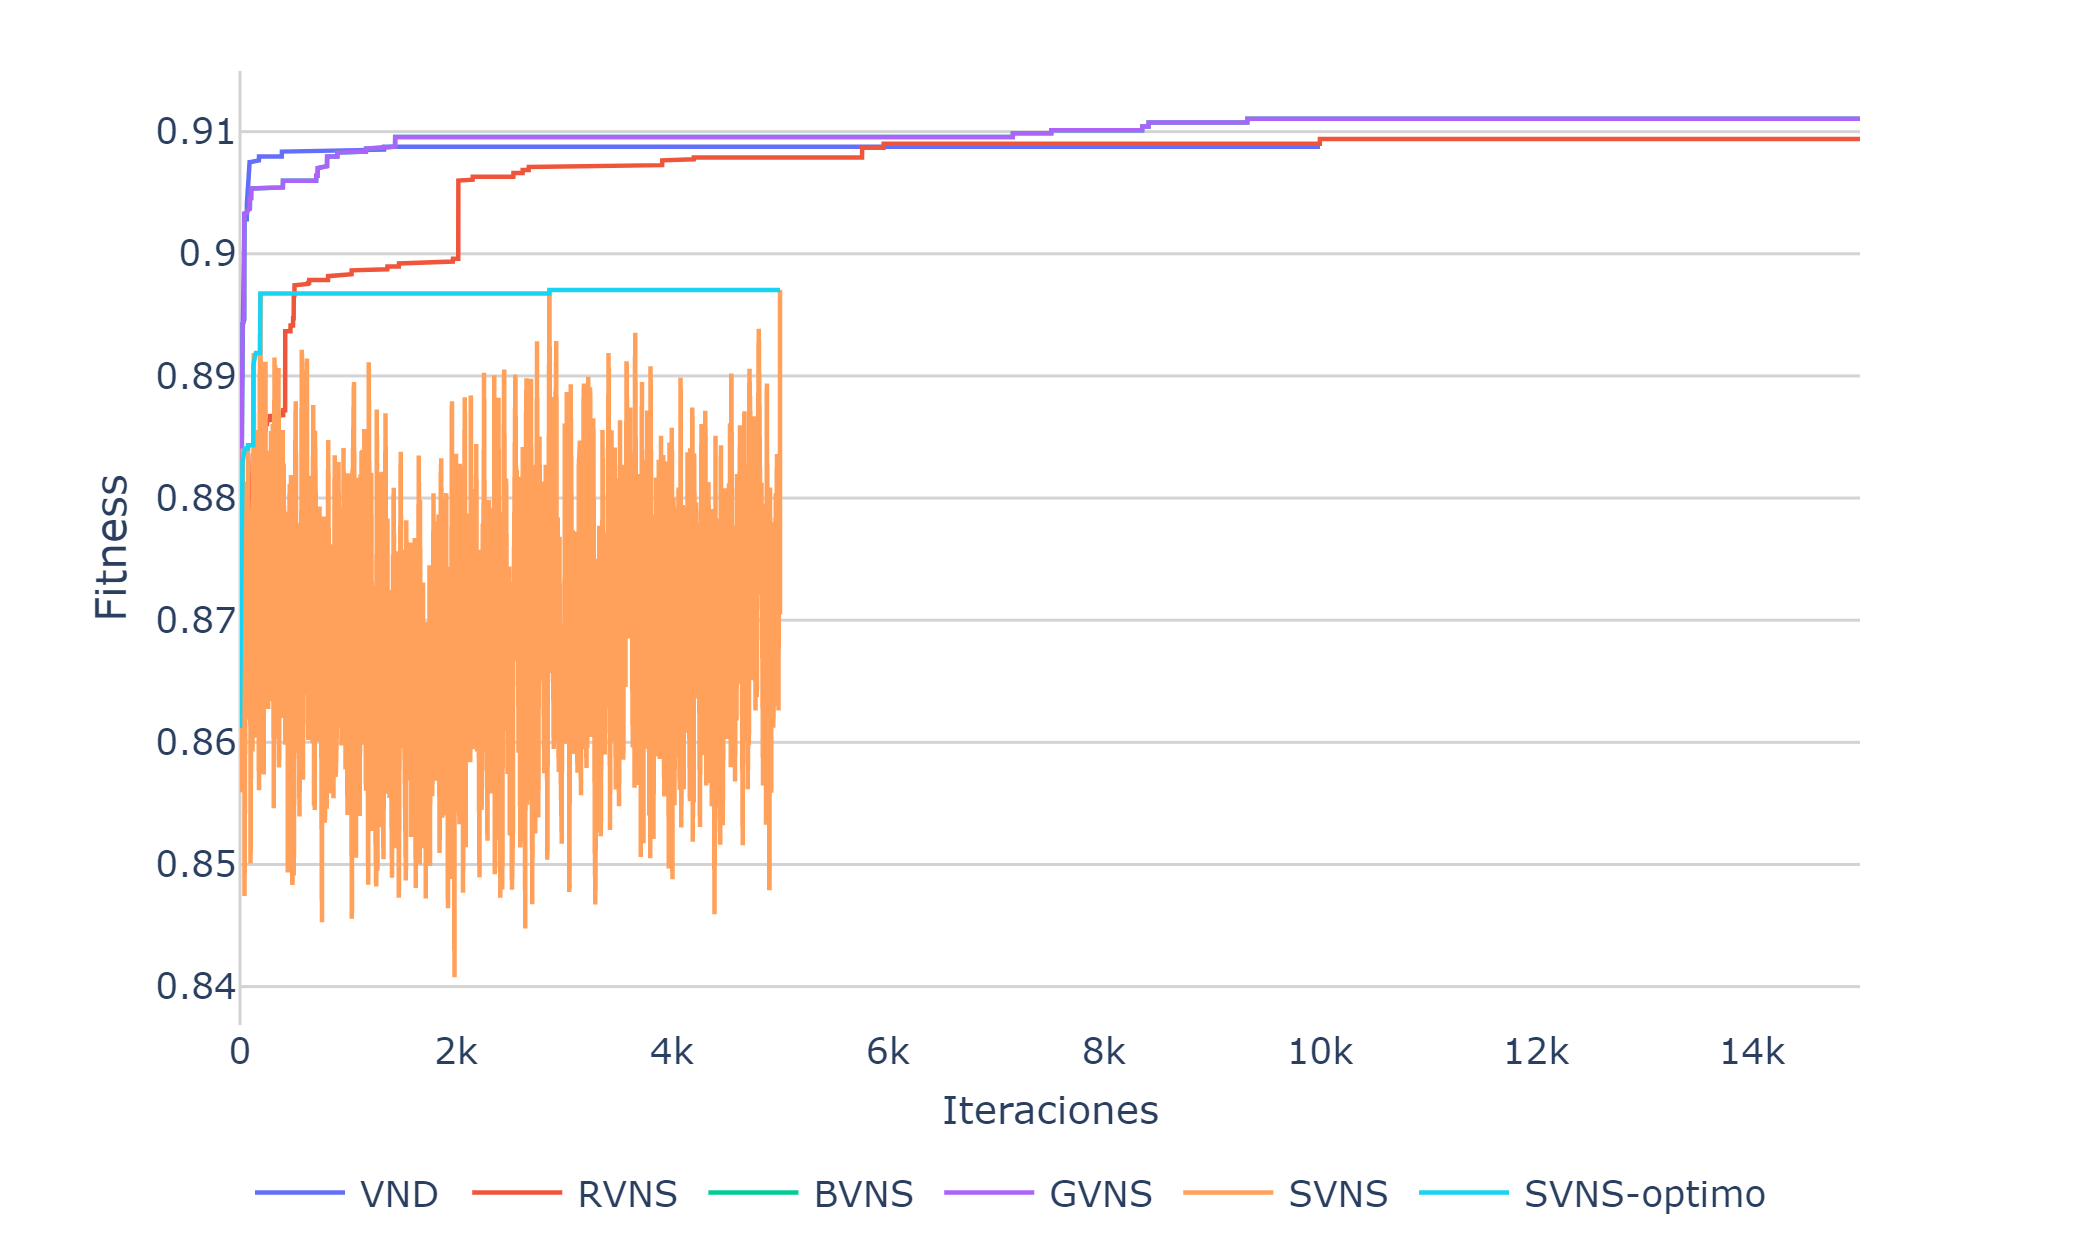
\includegraphics[width=\linewidth]{Caso4_comparativa-tipos-vns_iteracion}
		\caption{Caso 4}
		\label{fig:caso4comparativa-tipos-vnsiteracion}
	\end{subfigure}

	\begin{subfigure}{\linewidth}
		\centering
		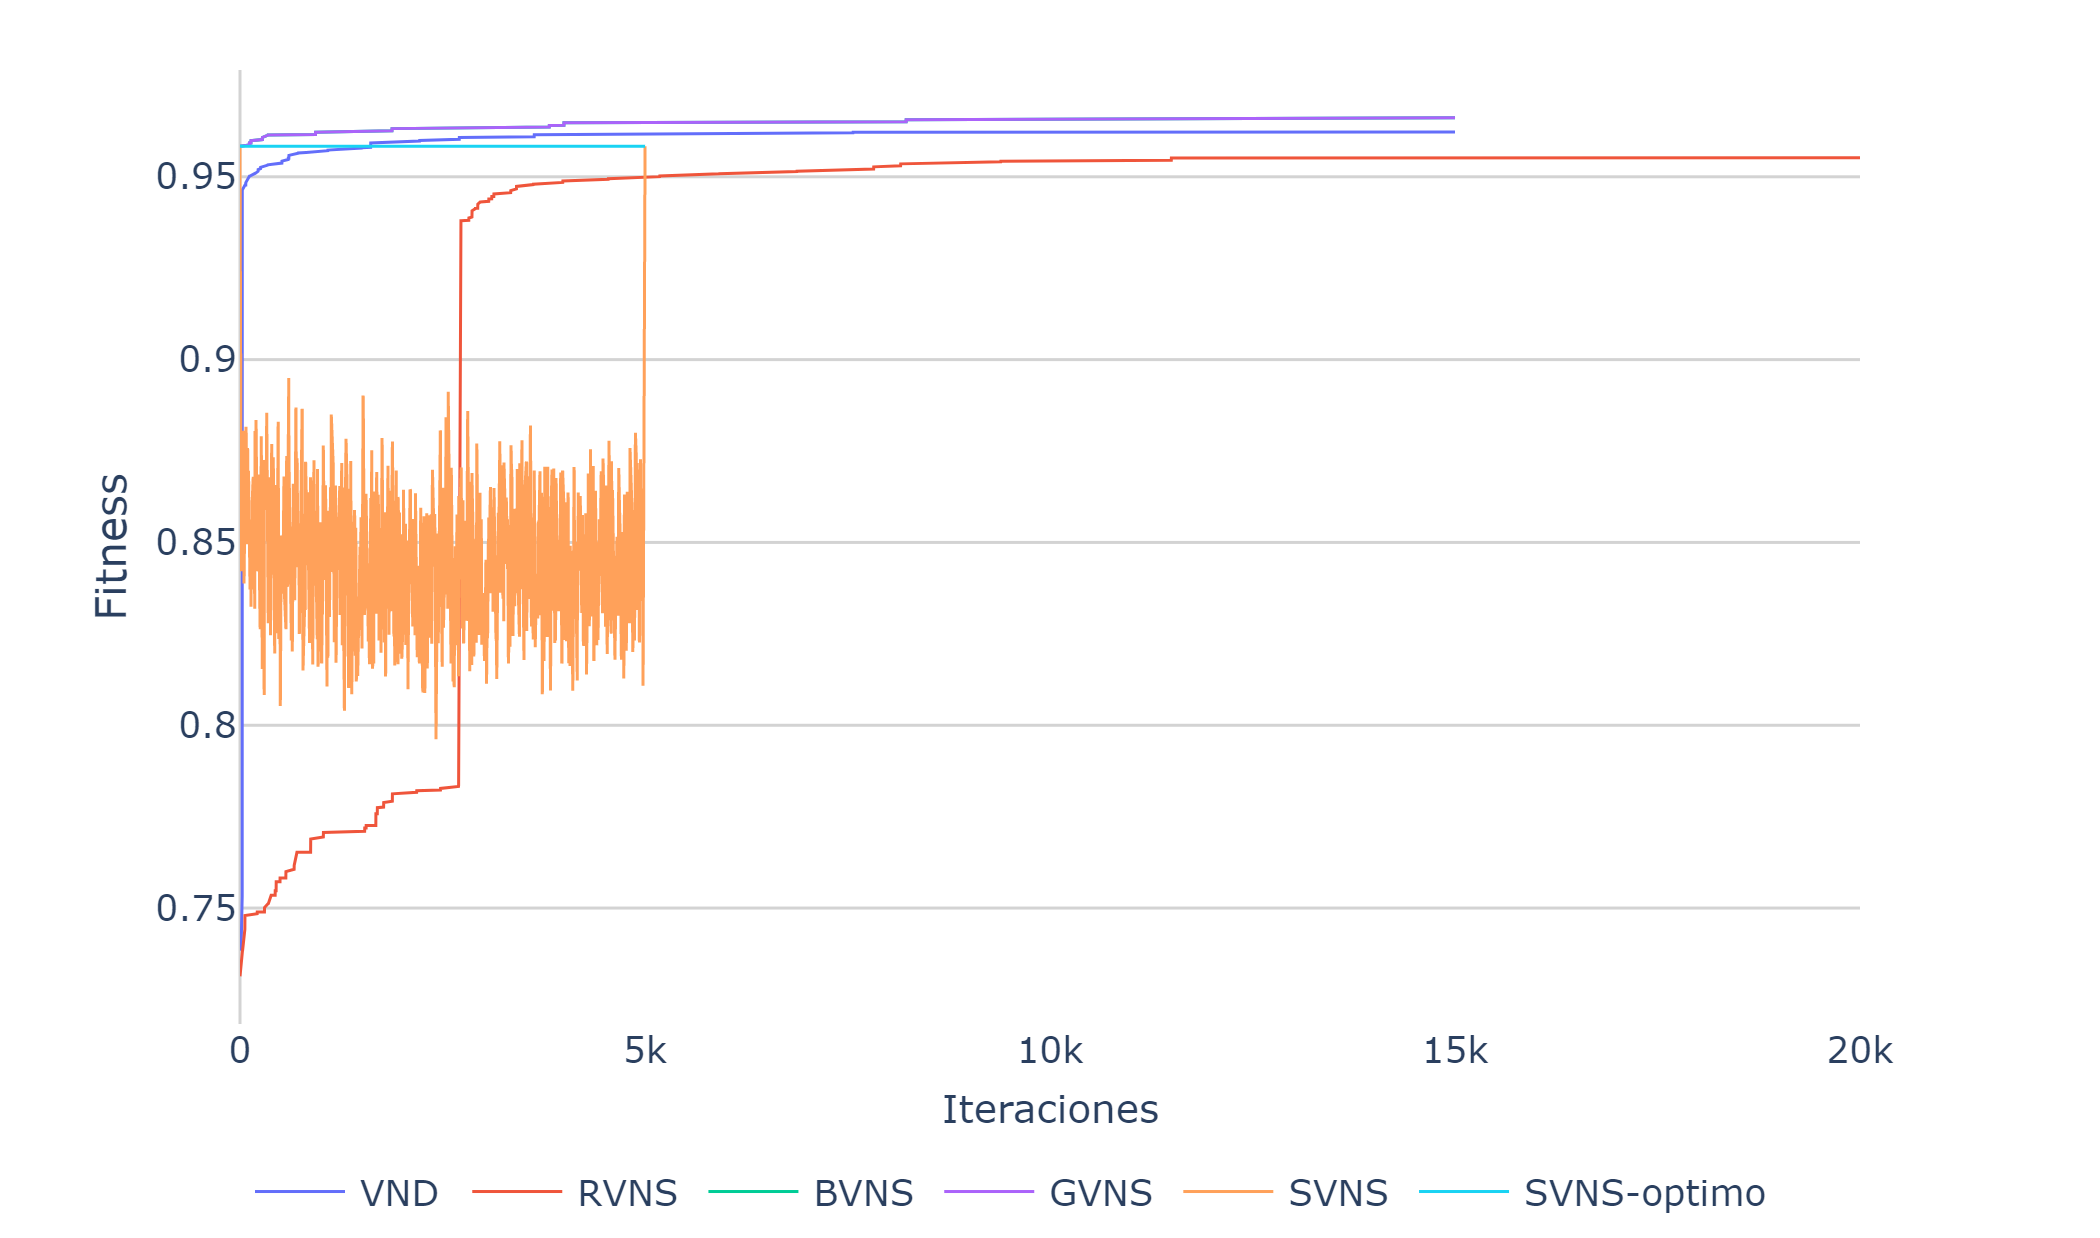
\includegraphics[width=\linewidth]{Caso9_comparativa-tipos-vns_iteracion}
		\caption{Caso 9}
		\label{fig:caso9comparativa-tipos-vnsiteracion}
	\end{subfigure}
	\caption{Evolución de cada \textbf{tipo de VNS} para una ejecución concreta del caso 4 y 9.}
	\label{fig:caso4y9comparativa-tipos-vnsiteracion}
\end{figure}

En cuanto al orden de los entornos, no hay una clara tendencia, sino que depende más bien del caso concreto. Sin embargo, la selección óptima de los mismos es claramente determinista, salvo en el caso 5 y 9. 
Una comparativa nos dice que la mejoría que aporta no es demasiado grande, del orden de una milésima (véase la \autoref{fig:caso5-naturaleza-entornos}) aunque para éste caso concreto, con la opción probabilística, el número de restricciones incumplidas en la solución final es menos dispersa que en la determinista, es decir, que la diferencia entre una ejecución u otra no es tan grande como en el caso de la determinista. No obstante, para el resto de casos ésta dispersión no sucede de una forma tan significativa.

\begin{figure}
	\centering
	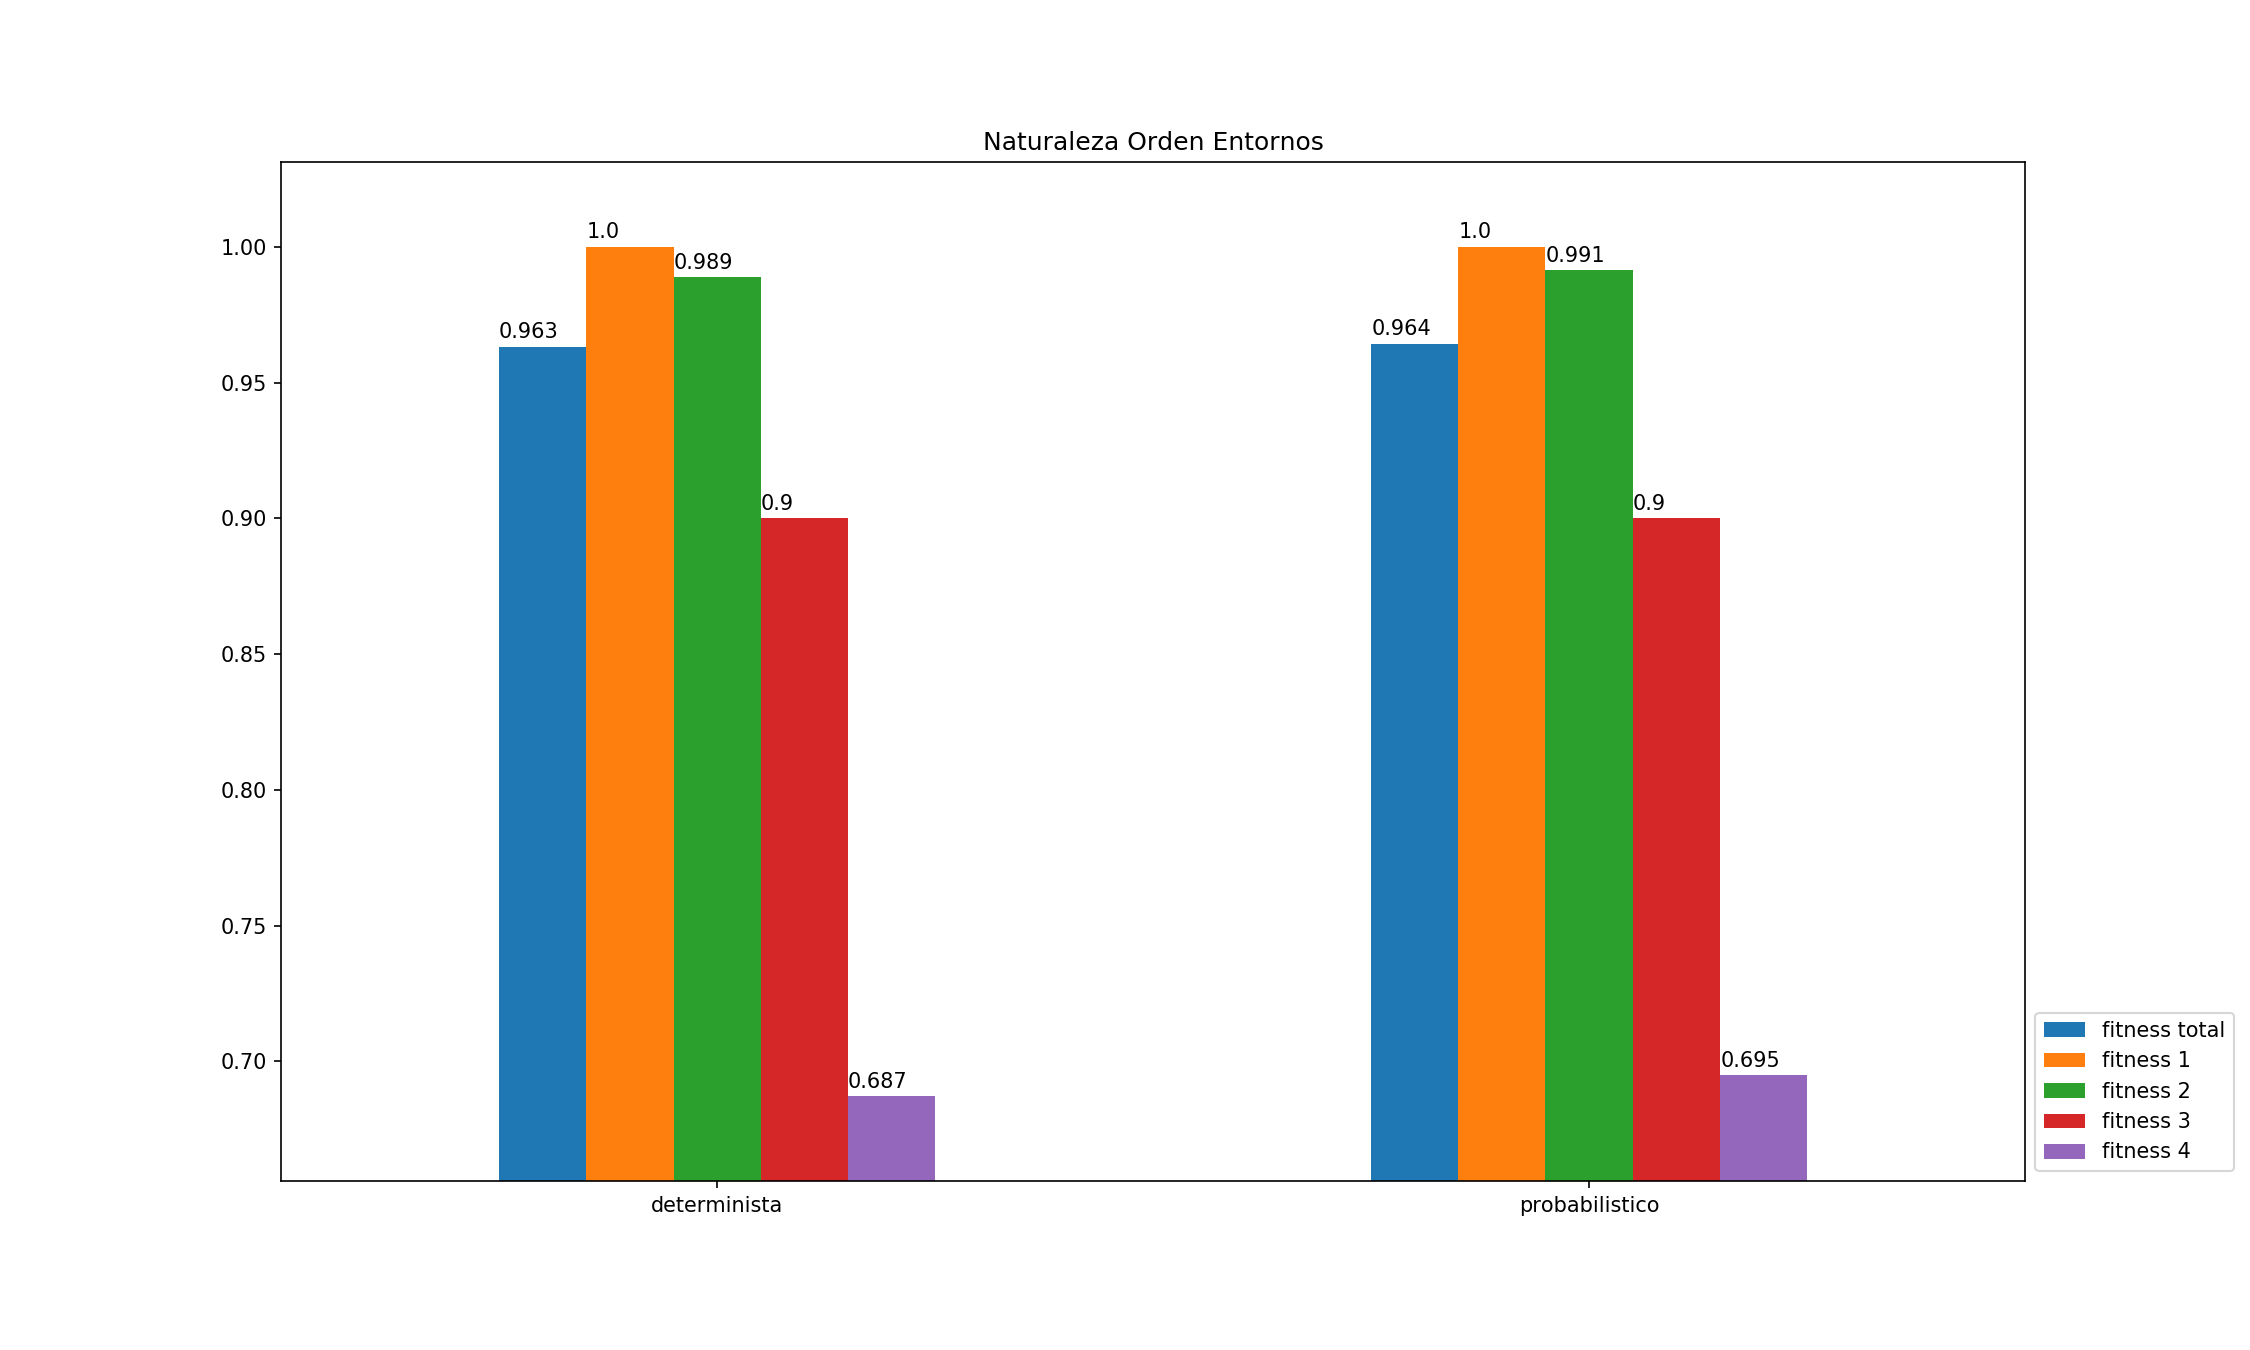
\includegraphics[width=1\linewidth]{caso5-naturaleza-entornos}
	\caption{Comparación desglosada por valor de cada objetivo para el \textbf{tipo de cambio de entorno} en el caso 5}
	\label{fig:caso5-naturaleza-entornos}
\end{figure}

En la \autoref{fig:caso4y9determinista-vs-probabilisticoiteracion} podemos observar la evolución de una ejecución comparando el desempeño de sistema para cambios de entorno de tipo determinista y probabilístico, una vez seleccionados los parámetros óptimos relativos a este último. Se aprecia cómo para el caso 9  (\autoref{fig:caso9determinista-vs-probabilisticoiteracion}), la diferencia es significativa: el probabilístico aporta lo suficiente como para considerarlo. Sin embargo, para el caso 4 (\autoref{fig:caso4determinista-vs-probabilisticoiteracion}) el tipo de cambio de entornos determinista supera al probabilístico pero por muy poca diferencia.l

\begin{figure}
	\begin{subfigure}{\linewidth}
		\centering
		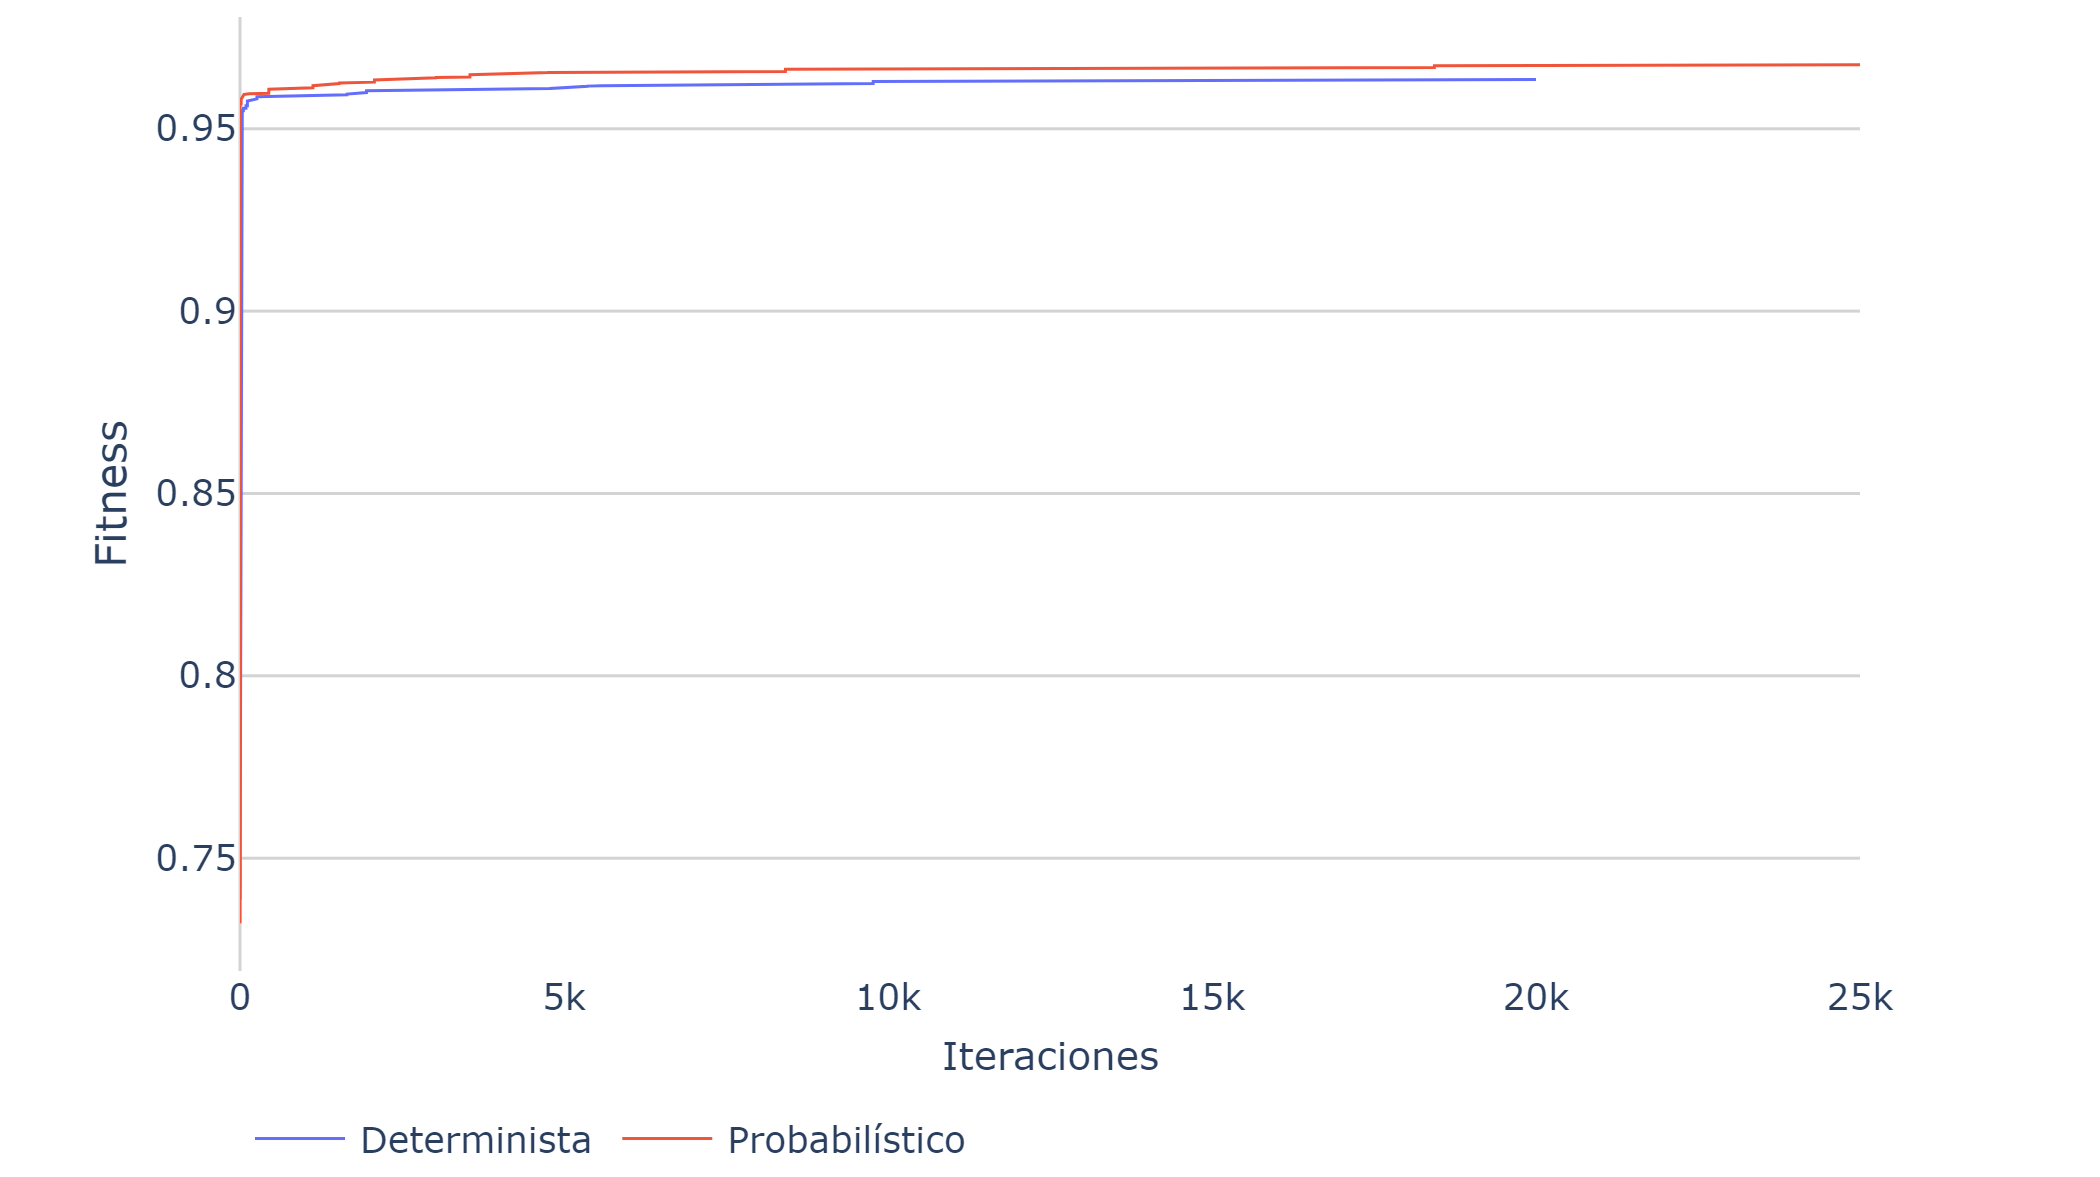
\includegraphics[width=1\linewidth]{capitulos/Capitulo5-Resultados-experimentales/recursos/Caso9_determinista-vs-probabilistico_iteracion}
		\caption{Caso 9}
		\label{fig:caso9determinista-vs-probabilisticoiteracion}
	\end{subfigure}

	\begin{subfigure}{\linewidth}
		\centering
		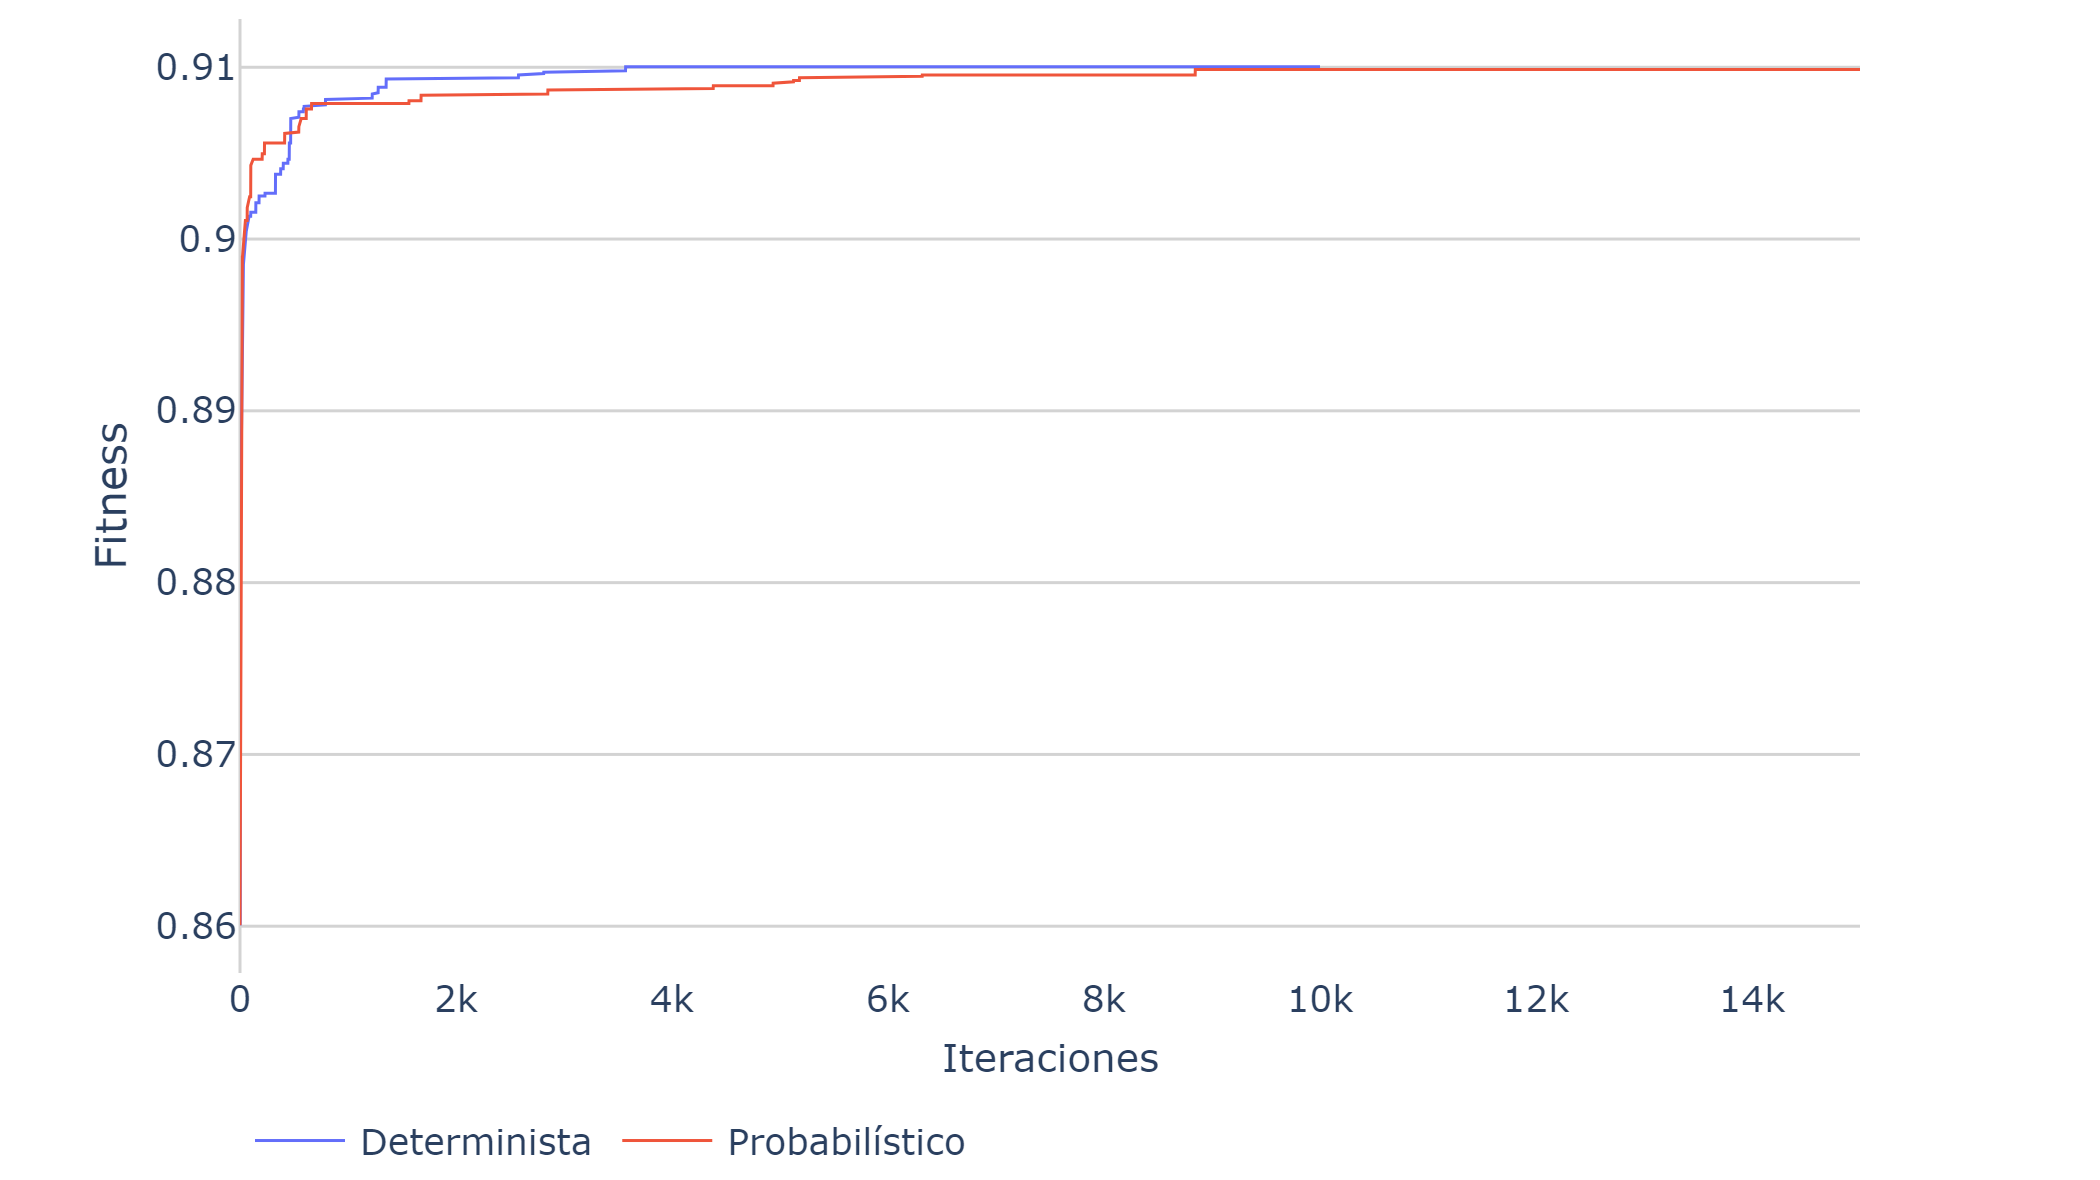
\includegraphics[width=1\linewidth]{capitulos/Capitulo5-Resultados-experimentales/recursos/Caso4_determinista-vs-probabilistico_iteracion}
		\caption{Caso 4}
		\label{fig:caso4determinista-vs-probabilisticoiteracion}
	\end{subfigure}
	\caption{Evolución del sistema para una ejecución concreta del caso 9 y 4 con \textbf{cambios de entorno} de tipo determinista o probabilistico.}
	\label{fig:caso4y9determinista-vs-probabilisticoiteracion}
\end{figure}


%Observamos que los parámetros óptimos que afectan a la modalidad probabilista de los entornos se adecuan al VNS en cuanto a que, por ejemplo emplear una probabilidad inicial de $0.7$ con una variación pequeña, en lugar de una probabilidad de 1, pues el número de iteraciones no es suficientemente grande como para que 

En cuanto a los demás parámetros, no hay diferencias importantes entre sí. En número de iteraciones que conforman el ciclo mínimo para comprobar la condición de parada se mueven entre $6\,000$ y $45\,000$.

La función de distancia aplicada para el \textit{SVNS} que mejores resultados alcanza es aquella que calcula el número de slots dispares entre ambas soluciones. Hemos observado que el valor del parámetro $\alpha$ óptimo oscila entre 0.5 y 2, y para tamaños superiores a 2, o bien deja de admitir soluciones peores, o bien se comporta de la misma forma que con otros valores inferiores. En la \autoref{fig:caso9comparativa-alphasiteracion0-5} podemos observar cómo se comporta la metaheurística \textit{SVNS} con diferentes $\alpha$ para el caso 9, si bien exploran de diferentes formas, no logran mejorar significativamente los resultados iniciales, aunque esto sí sucede aunque muy levemente, para el caso 3, como muestra la
\autoref{fig:Caso3_comparativa-alphas_iteracion}.

\begin{figure}
	\begin{subfigure}{\linewidth}
	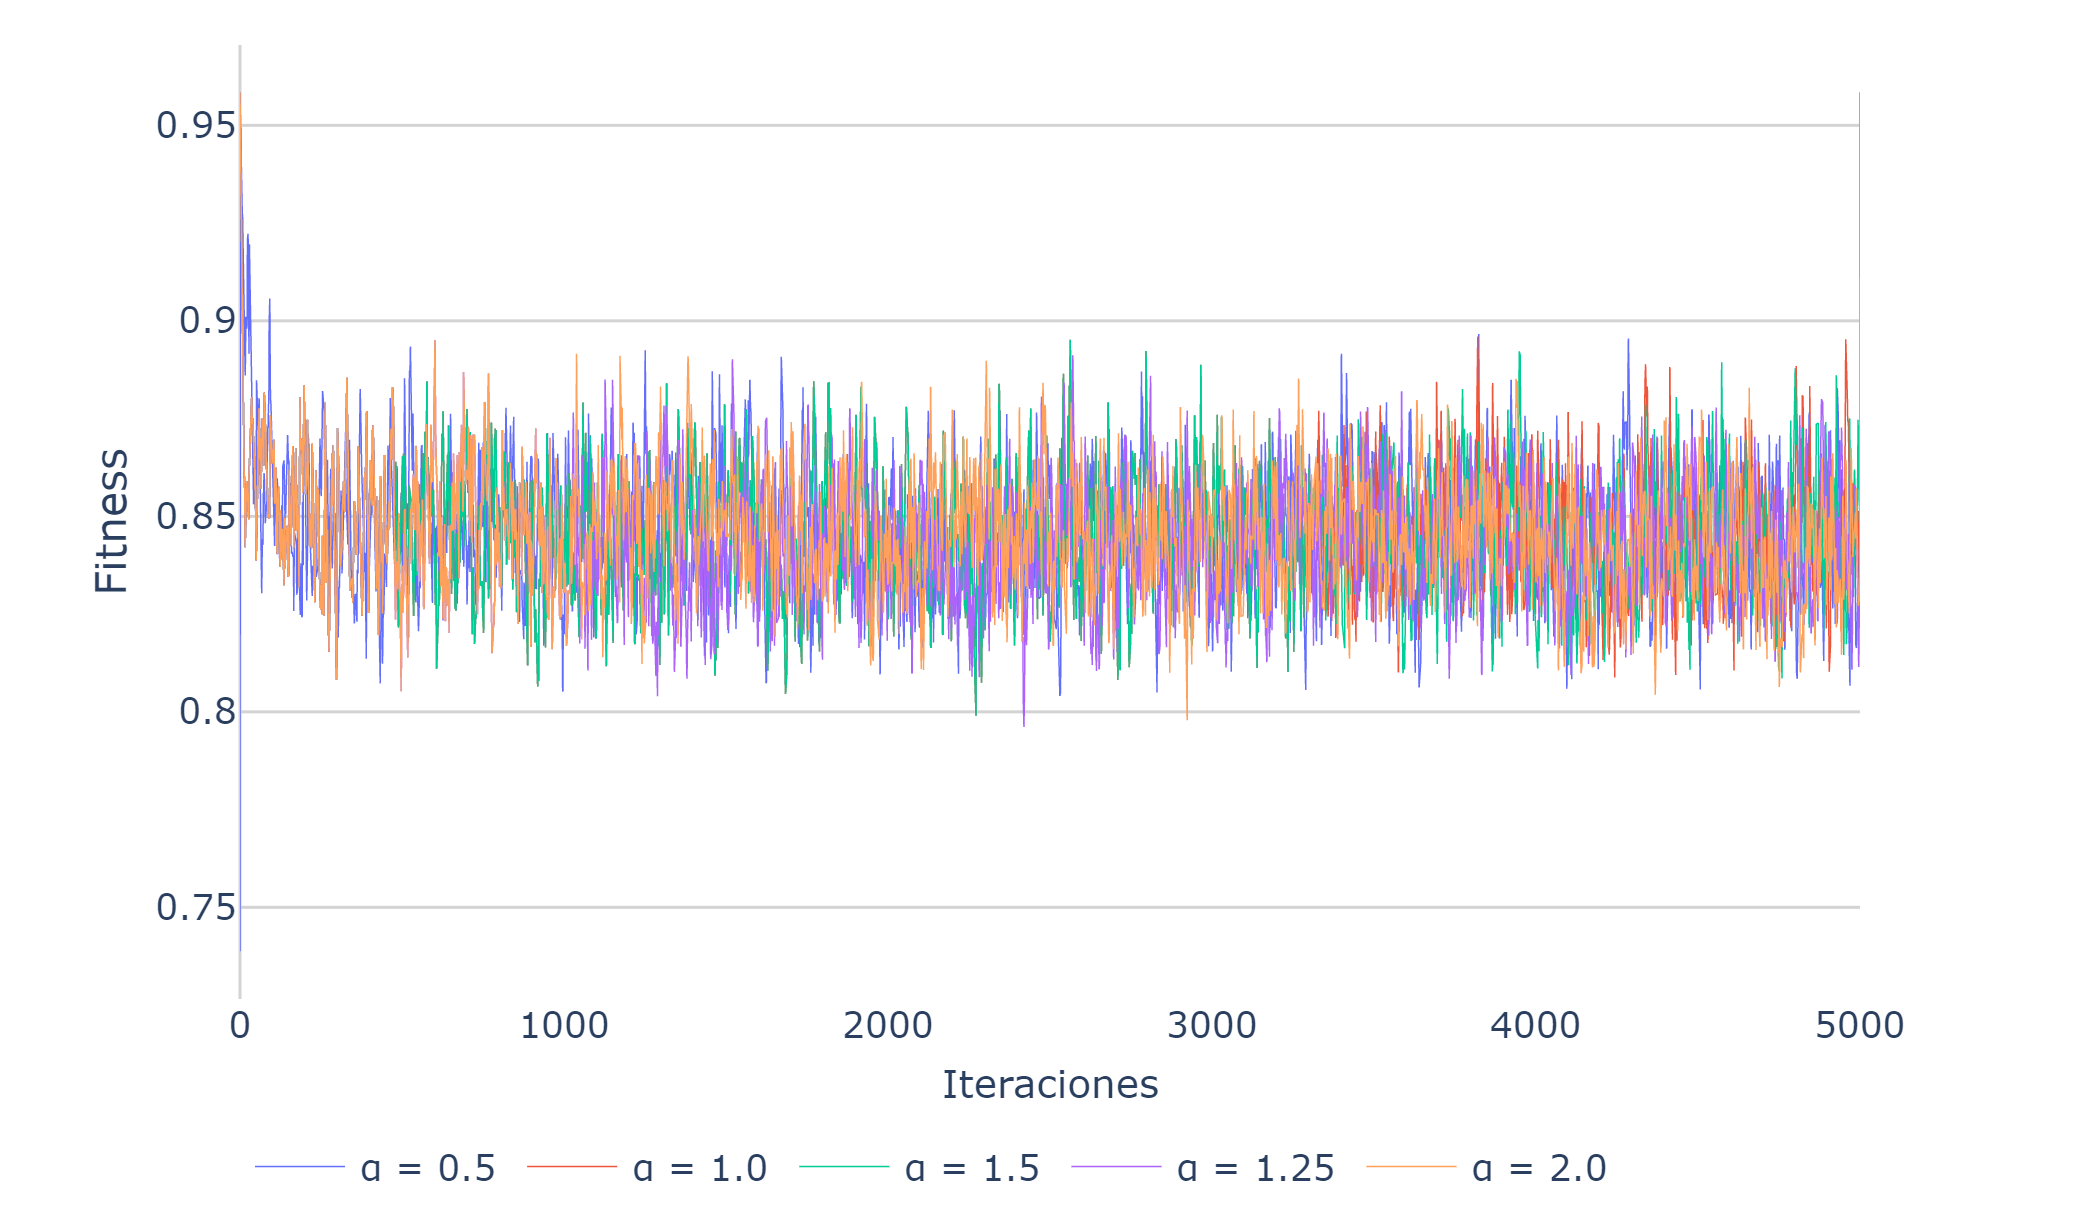
\includegraphics[width=\linewidth]{Caso9_comparativa-alphas_iteracion_0-5}
	\caption{Caso 9}
	\label{fig:caso9comparativa-alphasiteracion0-5}
	\centering
	\end{subfigure}

	\begin{subfigure}{\linewidth}
	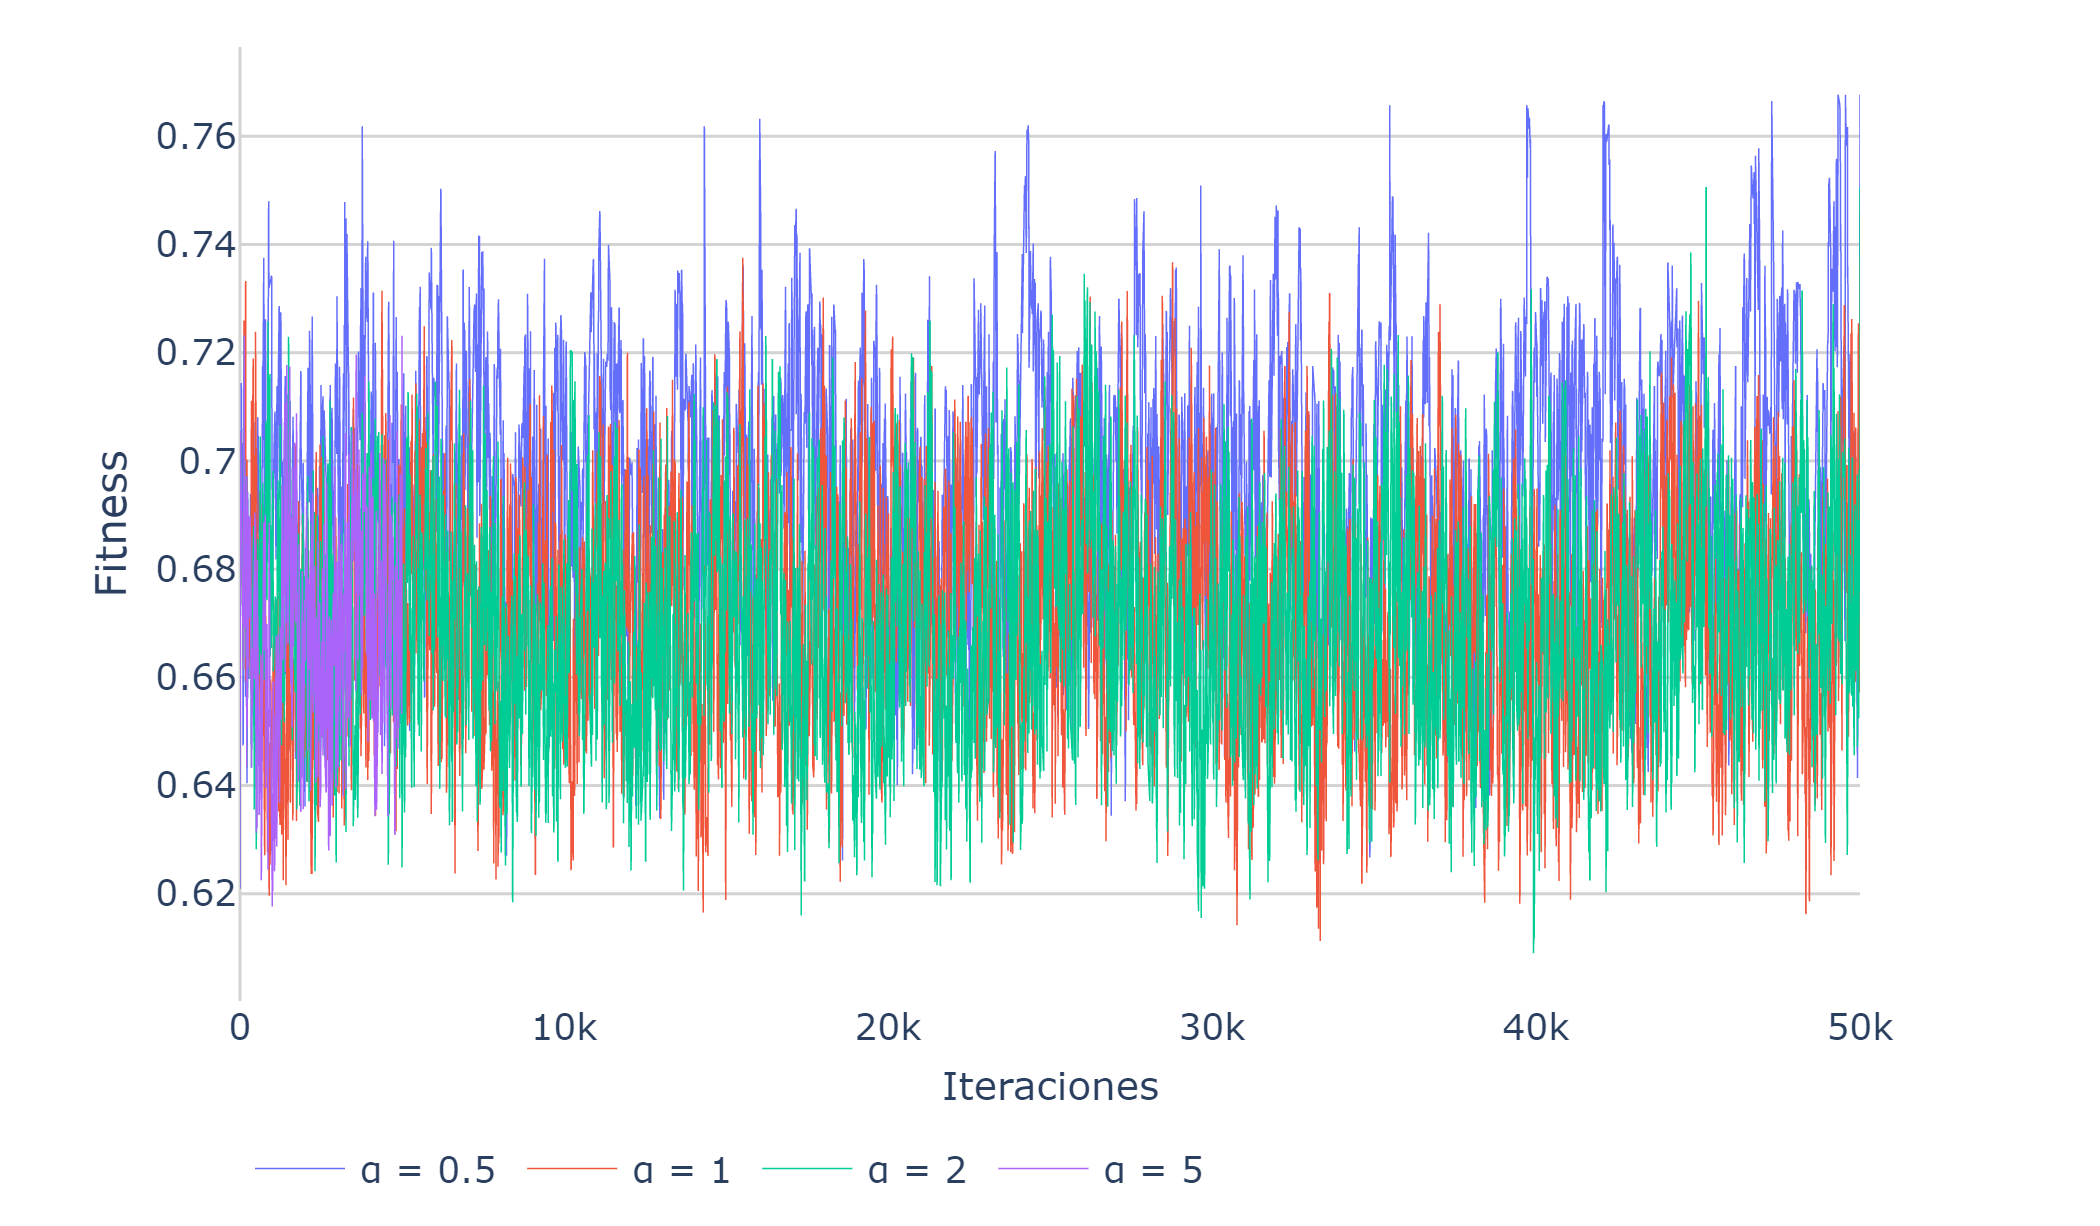
\includegraphics[width=\linewidth]{Caso3_comparativa-alphas_iteracion}
	\caption{Caso 3}
	\label{fig:Caso3_comparativa-alphas_iteracion}
	\centering
\end{subfigure}
	\caption{Evolución comparativa del desempeño del \textit{SVNS} con diferentes \textbf{alphas} para el caso 3 y el 9.}
\end{figure}

Para el caso 3, 

%A continuación describiremos algunas de las observaciones en mayor profundidad.
%
%\subsubsection{Comparativa de Tipos de VNS}
%
%Como se ha mencionado anteriormente, se han obtenido dos tipos de VNS con resultados especialmente mejores: el \textit{VND} y el \textit{BVNS}. Por lo general, la diferencia no es realmente grande, a excepción del caso 5, donde la diferencia es de 5 centésimas, sin embargo, en los casos indicados, el aporte sigue siendo significativo al conjunto, y la diferencia de tiempo

\subsection{Comparación de metaheurísticas}
Una vez ajustados todos los parámetros para sacar el máximo rendimiento del sistema, podemos compararlo con otros, y en este caso, se ha hecho una comparación de resultados con la metaheurística \sa{} (SA), definida en la \autoref{sec:3:metaheurística}. Recuérdese que se trata de la metaheurística empleada para el desarrollo del sistema \legacy{} y que fue adaptada a las nuevas condiciones y restricciones del sistema implementado en este TFM.

La \autoref{tabla} recopila los resultados para ambas metaheurísticas. Como podemos ver, % TODO . . . 

%\subsection{Otros experimentos}
%Lorem ipsum
